%% Sample chapter file, for use in a thesis.
%% Don't forget to put the \chapter{...} header onto each file.

\chapter{Description of the work undertaken}
\bibliography{thesis}
	\section{Discover}
	
During the discovery phase of the project the objective was to become familiar with the CEC environment, i.e. find out what tools are available and how they are being used and gather information about how to best contribute to the organisation. This was to be done while staying as open as possible, allowing any influences or ideas.

At the beginning of the project I had no knowledge about the operations within the Council or which departments would be involved. Some of the questions I wanted to answer included:
\begin{itemize}
\item Are there any activities in the Council similar to the scope of the project (or were there any in the past)?
\item Who would benefit from it and how to give those stakeholders an opportunity to be involved?
\item What questions (in terms of “channel shift”) are not answered in the Council?
At what level of abstraction should the analysis be conducted?
\item What IT systems/tools can be used in the project?
\item Who has the necessary understanding of the infrastructure and activities on the architectural level?
\item What else do I not know?
\end{itemize}

		\subsection{Meetings at the Council}
		
Initially the contact person from the Council was Sally Kerr. In response to my questions she arranged a meeting with an enterprise architect Neil Dumbleton. The purpose of the meeting was to give me an opportunity to ask questions regarding organisational structure as well as context of the project.

As it turned out, it was a first meeting in a series. There was no formalised documentation or central place with knowledge about on-going projects that was made available to the author. As a result, personal meetings were the only way to understand activity in the Council. Moreover, it was only thanks to good will of many employees at the City of Edinburgh Council that this was possible.

The diagram below shows all the people who I interacted with during the entire project. Connections between different actors represent how I got to know them. Circles with coloured backgrounds highlight people who I spoke with in this phase. Orange colour marks people related with University of Edinburgh, blue is for CEC employees. Level of a circle does not reflect a position in the Council’s structure - it is used solely for increasing legibility of the diagram.

\begin{figure}
\centering
     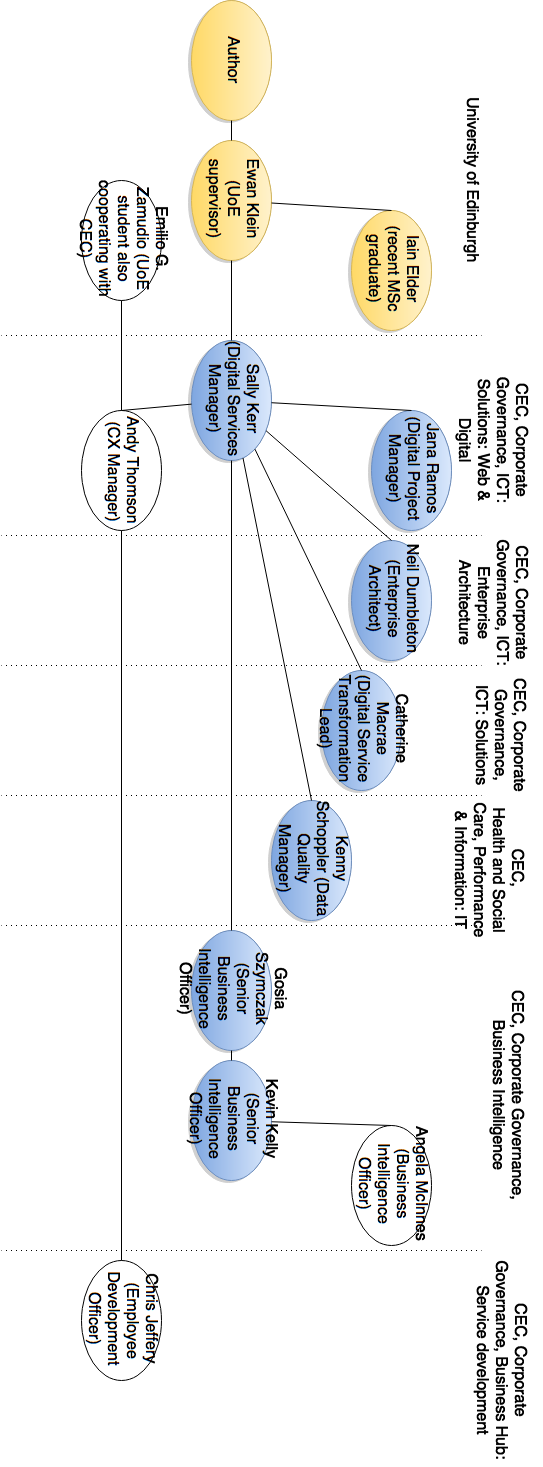
\includegraphics[height=\textheight]{Discovery_phase_people.png}
      \caption{CEC employees involved in the project.}
       \label{normal_case}
\end{figure}


From these meetings and discussions I gained a brief understanding of the situation at CEC. There was a big effort within the Council aiming at transforming the way services are being delivered and “Channel Shift” was a part of it. The outsourced ICT services in the Council were delivered by British Telecom starting from 2001 and the contract was set to end in 2016. In order to find a new service provider under revised conditions, a public tender was being held during the writing of this thesis. It considered “Channel Shift” as one of the significant enhancements of the Council’s operations. Final report suggesting the best bidder was submitted by the Finance and Resources Committee on third of August 2015 \citep{FinanceandResourcesCommittee2016}.

In summer 2014 a new CRM system was introduced called Oracle RightNow. It was replacing the old system called Capture. The deployment was part of the transformation. The system was used to capture information about all interactions with citizens and in some cases it meant that entries did not have all the values specified (due to the nature of an inquiry). The incompleteness of entries did not make them useless as they could still inform about things like level of use. The data captured has not been analysed from the angle described in this project (socio-economic insights) and it was confirmed that such analysis would be useful for the Council.

The transformation within the Council was also trying to centralise Business Intelligence capabilities. The BI department had a number of responsibilities and systems. One of those systems was called IBM Cognos. It was fully operational and a number of reports were generated and delivered to other stakeholders. However, the scale of deployment was still unclear and many departments were still figuring out the role the system would play in their operations. Many services required more digitisation and given the strategy, they could potentially use Cognos in the process. CRM data was an example of a dataset that was promising in providing valuable business insights.

Considering the above, the project would develop a piece of work that would increase know-how within the Council (in terms of using data analysis for designing services and interfaces), provide a “case study” and directly deliver business value to the organisation. The tools and datasets that could be used are described in the following sections.

		\subsection{CRM data}
		
The new system used at the Council was called RightNow and was provided by Oracle. It was a cloud service and the data in the system was available to CEC employees after registration (with staff number) and installation of the interface. The database consisted of a number of tables, e.g. “Answers” which was a “knowledge base for consultants”. The table used in the project was “Incidents” and it contained information about transactions initiated by citizens (issues reported by them through all channels). This choice was dictated by the scope of the project - de facto by preferences of the clients who were interested in better understanding of the usage patterns of citizens.

Unique Property Reference Number (UPRN) is a number uniquely identifying a household in Edinburgh and thus a person (or a family). Incidents table had a column named UPRN which provided information about who reported the issue. The Mosaic personas (introduced in the next section) were also using UPRN making it possible to link the two datasets. The table had dozens of columns containing information about things like channel used to report the issue, postcode where it was reported, date, Service Level Agreement (SLA).

The incidents table selected for this project (which is a part of the CRM database) apart from storing detailed information on issues reported by citizens provides means for tracking activity across different channels. Some enquires are just general questions and as a result, many entries do not have all values filled in. This enriches the dataset giving a fuller picture of what is happening, i.e. keeping a trace of all enquires.		
		
		\subsection{Mosaic UK Consumer and Demographic data}
		
Mosaic is a dataset created by Experian - credit reference agency. It provides insights about lifestyles and preferences of people across the United Kingdom. It identifies 14 social groups and a total of 57 types within those groups. It was built using more than 450 data variables and the sources include, but are not limited to \citep{Experian2014}:	

\begin{itemize}
\item Census
\item Open Data
\item OFCOM Broadband speeds
\item Higher Education Statistics Authority (HESA)
\item Electoral Roll
\item Council Tax property valuations
\item YouGov’s survey of consumers and their financial behaviour
\item British Crime Survey
\end{itemize}

It is highly detailed (e.g. food a person buys based on information from retailers) and granular (every household). It can be used as a numerical dataset (Cognos package) or a descriptive interpretation (Segmentation portal).

Since the portal is very useful in working with Mosaic data, after a recommendation from the author access was granted to Andy Thomson (one of the receivers of the reports).

Some of the information about a household available in Mosaic includes:

\begin{itemize}
\item Age of members of the household
\item Income
\item Spending structure
\item Property type
\item Contact channel preference
\item Education
\item Access to technology
\end{itemize}
	
For example, selected characteristics of group D, referred to as “Rural Reality”, include: rural locations, village and outlying houses, agricultural employment, affordable value homes, slow Internet speeds. People in this group are aged 66+, they have income of £20k- £29k, they live alone (or in “pseudo families”) and compared to the rest of the population are less likely to have children. They live in bungalows, named buildings or semidetached households in majority owned by them. Comparing to the rest of the population in the UK, they are half as likely to prefer being contacted via  mobile call (in contrary to a landline). Majority of them use “pay as you go” tariffs with mobile bill of 10 pounds or less, they read regional papers and are very likely to do groceries in Co-op and very unlikely to buy in Waitrose. Much bigger part of this group (compared to other groups in the UK) is likely to use e-mail monthly and not listen to music using mobile technologies. 

\begin{figure}
\centering
     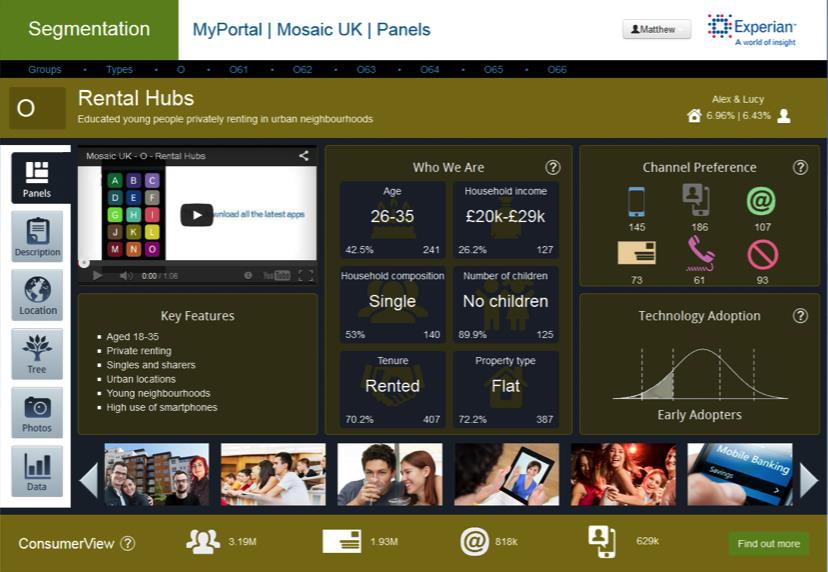
\includegraphics[width=\textwidth]{mosaic_segmentation_portal.jpg}
      \caption{Segmentation portal visualising Mosaic data \citep{Experian2014}.}
       \label{normal_case}
\end{figure}




		\subsection{IBM Cognos}
		
			\subsubsection{Introduction}
			
			\subsubsection{Working with IBM Cognos BI}

	\section{Define}

	\section{Develop}
	
	\section{Deliver}